\section{Processi organizzativi} \label{processi organizzativi}

	\subsection{Gestione di processo}

		\subsubsection{Scopo del processo}

			Il processo di gestione contiene le attività e i compiti generici che possono essere utilizzati da qualunque
			parte che deve gestire i rispettivi processi. Il manager è responsabile della gestione di prodotto,
			di progetto e dei compiti dei processi applicabili, come i processi di acquisizione, fornitura, sviluppo,
			funzionamento, manutenzione e di supporto.

			%Questo processo consiste nelle seguenti attività:
			%\begin{itemize}
			%    \item iniziazione e definizione dello scopo;
			%    \item pianificazione;
			%    \item esecuzione e controllo;
			%    \item verifica e valutazione;
			%    \item chiusura.
			%\end{itemize}

        \subsubsection{Comunicazione}\label{comunicazione}

            Questa sezione è dedicata all'illustrazione delle modalità di comunicazione che verranno 
            adottate dal gruppo \GroupName{} durante l'intera durata del progetto. Le comunicazioni 
            potranno essere interne al gruppo, o potranno coinvolgere soggetti esterni ed esso quali 
            \glossaryItem{Proponente}, \glossaryItem{Committenti} o altri \glossaryItem{stakeholder}.

            \myparagraph{Comunicazioni interne}

                Le comunicazioni interne avranno luogo tramite lo strumento di collaborazione aziendale Slack.

                %Andando ad illustrare e normare le conversazioni interne al team, va fatto presente che la maggior parte di esse avranno
                %luogo tramite lo strumento di collaborazione aziendale Slack}.
                Slack è stato preferito ad altri software di messaggistica per la possibilità di creare 
                canali tematici e per l'alta integrabilità con altri servizi utilizzati dal team nel 
                corso di questo progetto.
                All'interno del workspace Slack, i membri del gruppo dovranno comunicare nel rispetto dei 
                temi dei canali creati, avvalendosi anche di features quali @everyone, @channel, 
                @NomeUtente per l'invio di notifiche rispettivamente a tutti i soggetti interni al 
                gruppo, a quelli che partecipano alla conversazione o a un utente specifico.

                Il workspace Slack è suddiviso in canali specifici per permettere un corretto scambio di 
                idee e informazioni, inerenti solamente a determinate aree del progetto.
                %Il team ha quindi deciso di dividere le comunicazioni in canali abbastanza specifici da poter permettere un
                %corretto scambio di idee ed informazioni, inerenti solamente a determinate aree del progetto.
                I canali presenti nel workspace sono:

                    \begin{itemize}
                        \item \textbf{canali dedicati a servizi utilizzati}: questi sono spazi dedicati ad integrazioni
                        con altri servizi quali ad esempio Asana e \glossaryItem{GitHub}. Viene creato un canale dedicato ad ogni integrazione;
                        \item \textbf{canali dedicati alla documentazione}: questi sono spazi dedicati alla documentazione
                        scritta dal team. Anche qui viene creato un canale per ogni documento da redigere, ad esempio
                        sono presenti canali quali ``norme di progetto" e ``piano di qualifica". All'interno di ogni spazio
                        verranno discusse sia le attività di sviluppo, che di verifica ed approvazione;
                        \item \textbf{canali dedicati ad argomenti specifici}: dal canale riguardante incontri e comunicazioni
                        con soggetti esterni, al canale dedicato al materiale informativo, a canali per la discussione dei
                        capitolati d'appalto o della scelta di nome e logo del gruppo;
                        \item \textbf{general e random}: canali di default, dedicati a comunicazioni non riferibili ad un
                        singolo processo o ad una singola attività.
                    \end{itemize}

                    \begin{figure}[htbp]
                        \centering
                        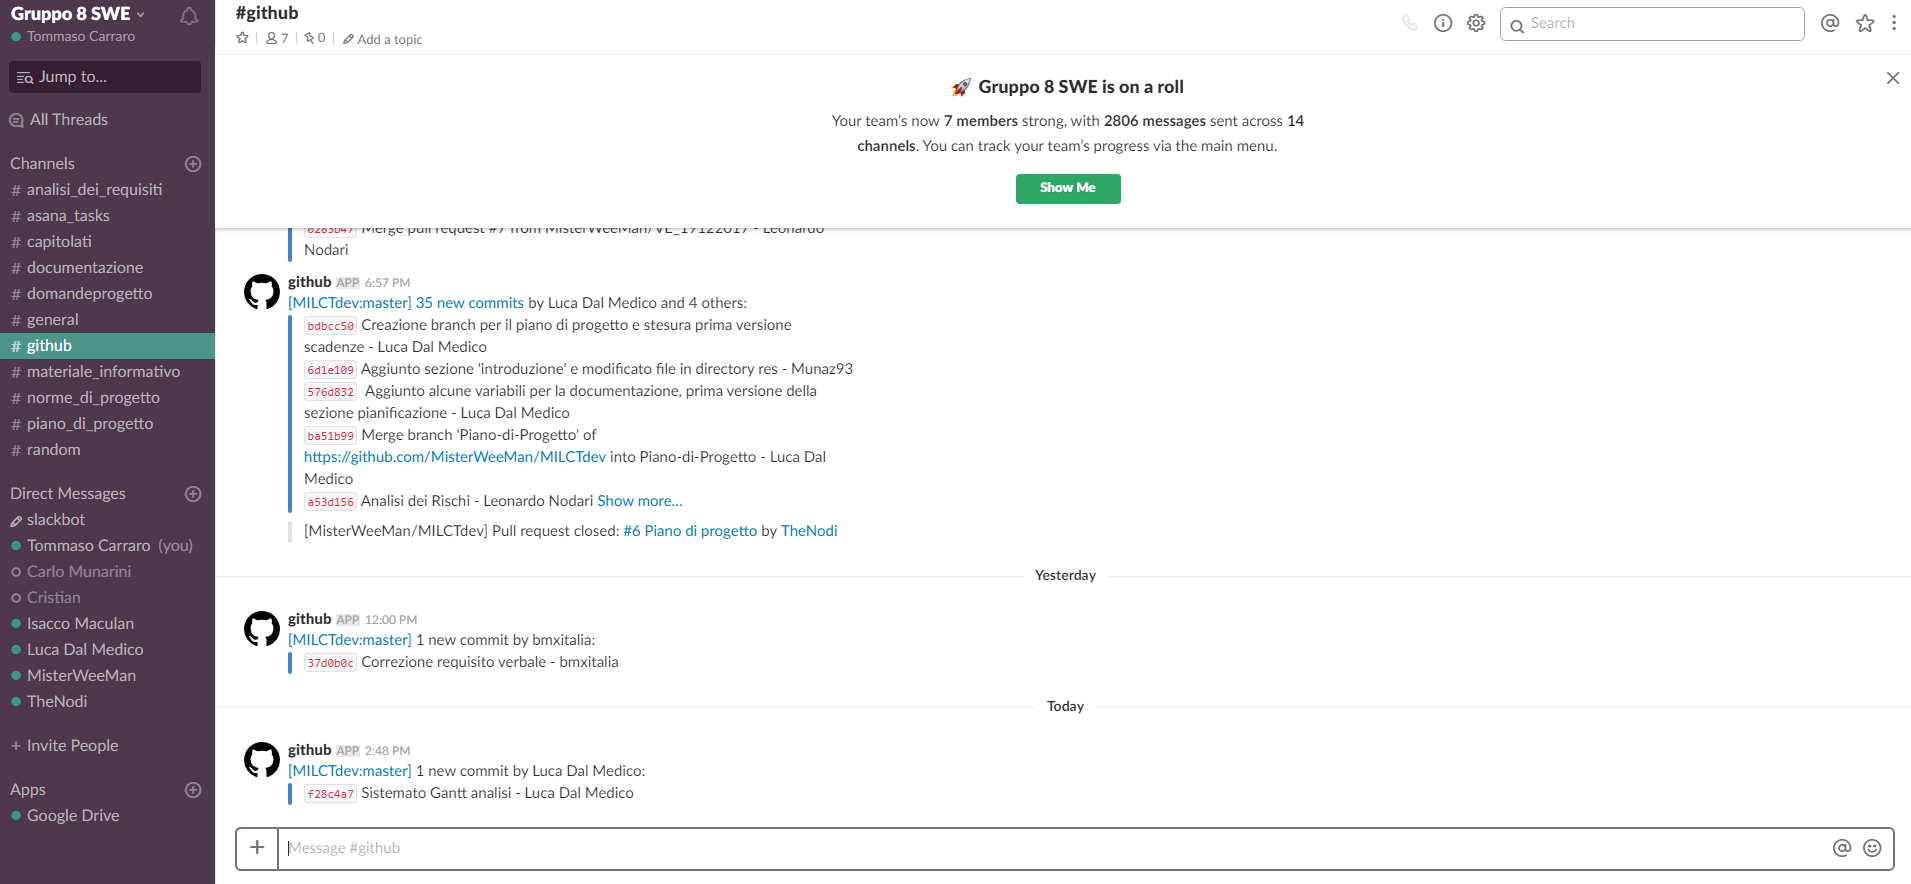
\includegraphics[scale=0.25]{./img/slack.png}
                        \caption[Slack]{Slack: strumento per la comunicazione del gruppo}
                    \end{figure}

			\myparagraph{Comunicazioni esterne} \label{comunicazione_esterna}

                Le comunicazioni intraprese con soggetti esterni al gruppo sono di competenza del Responsabile di Progetto
                che utilizzerà la casella di posta elettronica creata in fase di istituzione del team \GroupName{}: \GroupEmail{}.
                Il Responsabile di Progetto è quindi il soggetto incaricato dal gruppo per comunicare con i soggetti esterni,
                rappresentati da:

                    \begin{itemize}
                        \item \textbf{\Proponente{}}, nella figura di Proponente, raggiungibile all'indirizzo di posta elettronica: stefano.bertolin@iks.it;
                        \item \textbf{\Committenteinriga{}}, nella figura di Committenti, raggiungibili agli indirizzi di posta elettronica istituzionali.
                    \end{itemize}

                Tutti i membri del gruppo dovranno essere sempre aggiornati sulle conversazioni avvenute. Il compito
                di notificarli spetta al Responsabile di Progetto utilizzando l'apposito canale tematico all'interno del workspace Slack.

        \subsubsection{Incontri del team}

            Le riunioni del team, interne o esterne, verranno sempre organizzate in accordo con tutto il gruppo.
            L'organizzazione di esse spetta al Responsabile di Progetto.

            \myparagraph{Frequenza degli incontri}

                La frequenza è fissata ad almeno un incontro al mese, nel quale è richiesta la presenza di tutti i membri.

            \myparagraph{Verbali di riunione}

                Per ogni riunione verrà nominato un Segretario, a turno dal Responsabile di Progetto, il cui compito sarà
                redigere un verbale seguendo le norme della sezione 3.1.10.7.

\newpage

            \myparagraph{Decisioni e vincoli}

                Il numero minimo di membri richiesto per rendere valido un incontro è cinque. Tale numero impone una
                collaborazione tra gli elementi del team ed è sufficientemente grande a garantire equità nelle decisioni prese.
                Nel caso di riunioni straordinarie, il ``quorum" si abbassa a tre ma le decisioni prese dovranno essere
                riviste nell'incontro successivo.
                Ogni decisione verrà presa a maggioranza e, nel caso di parità di voti, la parola spetterà al
                Responsabile di Progetto che, dapprima si presterà nel ruolo di mediatore e, nel caso di fallimento
                delle trattative, dovrà prendere lui stesso una decisione.

        \subsubsection{Ruoli di progetto}

            Vista la natura didattica del progetto, nell'arco dell'intera durata dello stesso, ogni soggetto coprirà almeno
            una volta ognuno dei ruoli che verranno di seguito illustrati.
            Ogni membro dovrà svolgere le attività assegnate al ruolo ricoperto, come organizzato e stabilito dal documento
            \vPianoDiProgetto{}.
            Al fine di non minare la qualità di prodotto all'interno del \vPianoDiProgetto{} verranno pianificati dei turni
            tali da non creare conflitti d'interesse. Un esempio di conflitto d'interesse potrebbe essere dover verificare
            qualcosa che si era precedentemente scritto.
            I ruoli che verranno ricoperti dai membri del team sono illustrati nelle sezioni sottostanti.

            \myparagraph{Responsabile di progetto}

                Il Responsabile di progetto, anche chiamato Project manager, è una figura di estrema importanza all'interno
                del team in quanto su di lui ricadono responsabilità di pianificazione, gestione, controllo e coordinamento.
                Il Project manager rappresenta inoltre \GroupName{} all'esterno del gruppo in quanto intrattiene rapporti
                con Committente e Proponente. In sunto, egli:

                    \begin{itemize}
                        \item gestisce, controlla e coordina risorse, umane e non;
                        \item gestisce, controlla e pianifica le attività di progetto;
                        \item analizza e gestisce i rischi;
                        \item approva documenti.
                    \end{itemize}

                Questa figura è presente durante tutta la durata del progetto.

            \myparagraph{Amministratore}

                L'Amministratore è una figura di supporto che mette a disposizione strumenti e tecnologie per perseguire
                qualità ed efficienza all'interno dell'ambiente lavorativo.
                Egli quindi non opera scelte gestionali ma:

                    \begin{itemize}
                        \item monitora e lavora per il perseguimento della qualità di prodotto;
                        \item ricerca strumenti per l'automazione di attività, processi e compiti;
                        \item supervisiona e si adopera per la gestione del versionamento e l'archiviazione della documentazione;
                        \item controlla versioni e configurazioni del prodotto software;
                        \item norma l'utilizzo degli strumenti utilizzati durante il progetto.
                    \end{itemize}

            \myparagraph{Analista}

                L'Analista è una figura che non sarà sempre presente durante il progetto, ma di estrema importanza per i compiti svolti.
                Egli ha l'onere di comprendere appieno il dominio del problema e, tramite le sue azioni, vincolerà anche
                l'operato di alcuni ruoli, quali, ad esempio, i Progettisti.
                I suoi compiti sono:

                    \begin{itemize}
                        \item studiare il dominio del problema ed il problema stesso, definendone complessità e requisiti;
                        \item redigere documenti quali Analisi dei Requisiti e Studio di Fattibilità.
                    \end{itemize}

            \myparagraph{Progettista}

                Il Progettista è colui che, partendo dallo studio e dai vincoli posti dall'Analista, definisce una
                soluzione che soddisfi i requisiti.
                Egli è responsabile degli aspetti tecnologici e tecnici del progetto e dovrà:

                    \begin{itemize}
                        \item produrre una soluzione attuabile al problema;
                        \item sviluppare un'architettura che sfrutti soluzioni note ed ottimizzate che portino ad un prodotto
                        stabile e manutenibile.
                    \end{itemize}

            \myparagraph{Programmatore}

                Il Programmatore è la figura che provvederà alla codifica della soluzione, studiata e spiegata dal Progettista.
                Egli in particolar modo esegue queste operazioni:

                    \begin{itemize}
                        \item codifica la soluzione descritta dal Progettista nel rispetto di documenti, tra i quali le Norme di Progetto;
                        \item crea o gestisce componenti di supporto per la verifica e la validazione del codice.
                    \end{itemize}

                Questa figura ha inoltre il compito di manutenere il codice del prodotto e redigere un eventuale Manuale Utente.

            \myparagraph{Verificatore}

                Il Verificatore è una figura che è presente sin dalle prime fasi del progetto e lo sarà per tutto il ciclo di vita del software.
                Egli si focalizza sui processi e, grazie alla sua conoscenza delle \NormeProgetto{}, garantirà che essi
                siano conformi alle norme e alle attese.
                Il \Verificatore{} controlla quindi che:

                    \begin{itemize}
                        \item ogni stadio del ciclo di vita del prodotto sia conforme al \vPianoDiQualifica{};
                        \item ogni processo sia eseguito nel rispetto delle \vNormeDiProgetto{}.
                    \end{itemize}

        \subsubsection{Strumentazione}

        \myparagraph{Strumenti di comunicazione}

            Per la comunicazione i componenti del gruppo dovranno utilizzare Slack (di cui si è ampiamente parlato in
            precedenza) e Gmail.
            %Per quanto riguarda la parte relativa alla comunicazione, il team utilizzerà strumenti quali Slack e
            %\glossaryItem{Gmail}, già citati nella sezione §\ref{comunicazione}.
            %Dello strumento di collaborazione aziendale, Slack, si è già discusso in precedenza.; il secondo servizio
            %invece è Gmail, famoso servizio di posta elettronica fornito da Google, che viene usato dal team
            %nell'intraprendere conversazioni con soggetti esterni al gruppo.

        \myparagraph{Strumenti di condivisione}

            Come strumento di condivisione il team dovrà utilizzare Google Drive, servizio cloud based,
            per il quale è presente un'integrazione Slack, che permette al gruppo un rapido scambio di documenti e file.
            %Un altro servizio utilizzato dal team è \glossaryItem{Google Drive}, servizio cloud based, per il quale è
            %presente un'integrazione Slack, che permette al gruppo un rapido scambio di documenti e file.

        \myparagraph{Strumenti di coordinamento}

            Il team utilizzerà Asana come strumento di coordinamento orientato al ticketing.
            %Il sistema adottato per la coordinazione dei membri del team, mediante l'assegnazione di \glossaryItem{task}, è Asana.
            Alcune delle funzionalità che questo strumento offre sono:

                \begin{itemize}
                    \item creare un task, eventualmente inseribile in una ``sezione" o all'interno di un altro task;
                    \item indicare una persona a cui viene assegnato il task/sottotask;
                    \item indicare una data di scadenza del task, andando così a popolare un calendario utile al coordinamento;
                    \item inserire una descrizione del task e creare una conversazione relativa al task stesso.
                \end{itemize}

            %Con il passaggio alla versione pro, per il quale il team ha provveduto ad effettuare richiesta,
            %le possibilità si amplieranno e permetteranno anche la creazione di propedeuticità tra i task.
            %Questo strumento è stato inoltre integrato in un apposito canale tematico all'interno del workspace Slack,
            %per facilitare la notifica di nuovi eventi.

                \begin{figure}[htbp]
                    \centering
                    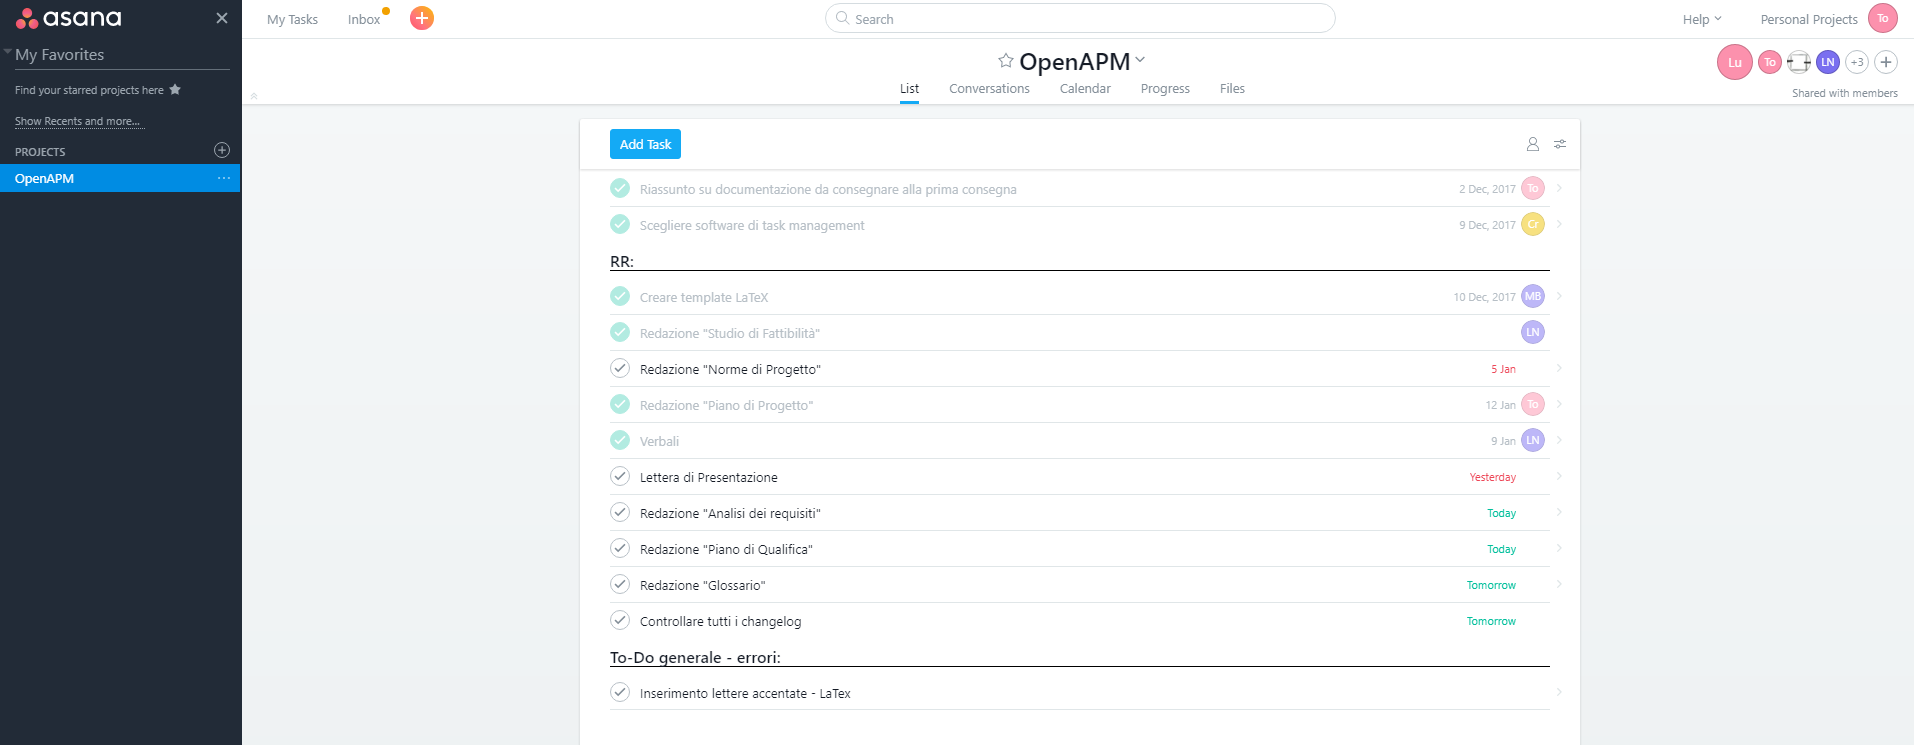
\includegraphics[scale=0.25]{./img/asana.png}
                    \caption[Asana]{Asana: strumento utilizzato dal gruppo per il coordinamento del progetto didattico}
                \end{figure}

        \myparagraph{Strumenti di versionamento}

            Per il salvataggio e versionamento dei file il team utilizzerà una repository su GitHub, il quale
            si basa sul sistema di versionamento Git.
            %La scelta è caduta su questo servizio, data la familiarità di diversi membri del gruppo con lo stesso.
            La repository contenente la documentazione, ha la seguente struttura (cartelle), alla quale i membri dovranno attenersi:

                \begin{itemize}
                    \item \textbf{LatexLayout}: contenente file per l'agevolazione della scrittura e della creazione
                    dei documenti in \LaTeX{};
                    \item \textbf{NOMEREVISIONE}: all'interno di queste cartelle saranno presenti documenti,
                    suddivisi nelle directory INTERNI/ESTERNI, che ospitano i file \LaTeX{} e .pdf di ogni singolo tipo di documento.
                \end{itemize}

            Anche questo strumento è stato integrato nel workspace Slack, per favorire la notifica di nuovi eventi al gruppo.

		\myparagraph{Sistemi operativi}

			Data la mancata presenza di requisiti che impongano restrizioni sul sistema operativo da utilizzare,
			i membri del team potranno indistintamente usare sistemi Windows, MacOSX o Linux.

	\newpage

    \subsection{Formazione del personale}
    
    		\subsubsection{Scopo del processo}

		Il processo di formazione è un processo per fornire e mantenere personale qualificato. L'acquisizione, la fornitura,
		lo sviluppo, il funzionamento e la manutenzione di prodotti software dipende anche dalla preparazione e della
		competenza del personale. Per cui, è imperativo che il processo di formazione del personale deve essere pianificato e
		implementato in anticipo in modo che il personale sia sempre preparato e disponibile a lavorare in maniera efficiente
		ed efficace sul prodotto software.

		\subsubsection{Attività}

        Ogni membro studierà individualmente per essere preparato alla realizzazione delle varie parti del progetto.
        Saranno attribuiti dei task relativi allo studio di materiale complesso necessario allo svolgimento del progetto
        come ad esempio ``imparare ad utilizzare il linguaggio \LaTeX{}".